\documentclass[a4paper,10pt]{article}
\usepackage[utf8]{inputenc}
\usepackage{graphicx}


%opening
\title{Rapport du projet de probabilités et théorie des erreurs}
\author{Clément Tamines}

\begin{document}

\maketitle

\newpage

\tableofcontents

\newpage

\section{Introduction}

\subsection{Énoncé du problème}
L'énoncé du problème est le suivant :
\begin{quote}
On a essayé de caractériser les missmatch liés aux tailles de mémoires caches. 
Pour cela, on a mesuré les temps d'attente en millisecondes pour trois types de technologie ram. 
On demande si les temps d'attente sont significativement différents ? Justifier votre réponse.
\end{quote}

\subsection{Analyse du problème}
Nous devons comparer les trois types de technologie et dire si les temps d'attentes sont significativement différents.
Nous devons donc comparer les temps d'attente pour les trois différentes technologies pour vérifier cela.

Intuitivement, nous pourrions simplement comparer les mesures et vérifier les différences entre chaque mesures pour une taille donnée ou simplement
comparer les temps maximum d'attente de chaque technologie et prendre le plus petit (la technologie qui a les temps d 'accès les plus courts).
Cependant, ceci n'est pas la bonne façon de faire car nous disposons de plusieurs mesures qui peuvent changer selon plusieurs facteurs (par exemple la donnée à accéder).
Nous allons donc utiliser les méthodes vues au cours pour prédire l'efficacité de chaque technologie et ensuite les comparer. Nous commencerons cependant avec analyse naïve des données.

\subsection{Fichier de données}
Le fichier de données contenait quatre colonnes. La première donne la taille de la mémoire et les trois autres des temps d'attente en millisecondes.
Pour chaque taille donnée, nous avons 100 mesures fournies ce qui forme donc 10 paquets de 100 données par technologie.

\subsection{Analyse naïve des données}

Nous allons maintenant analyser naïvement les données. Pour cela nous allons les visualiser graphiquement et tenter de déterminer si la différence entre chaque
technologie est significative. Nous visualisons ici le temps d'attente en fonction de la taille de la mémoire.
\\
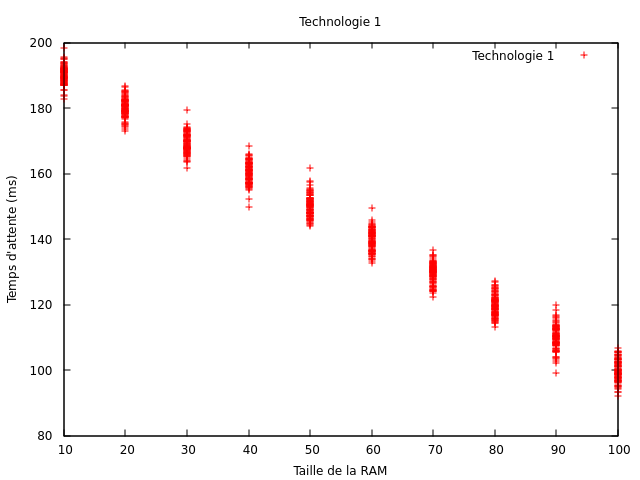
\includegraphics[scale=0.6]{img/techno1_plot.png}
\\
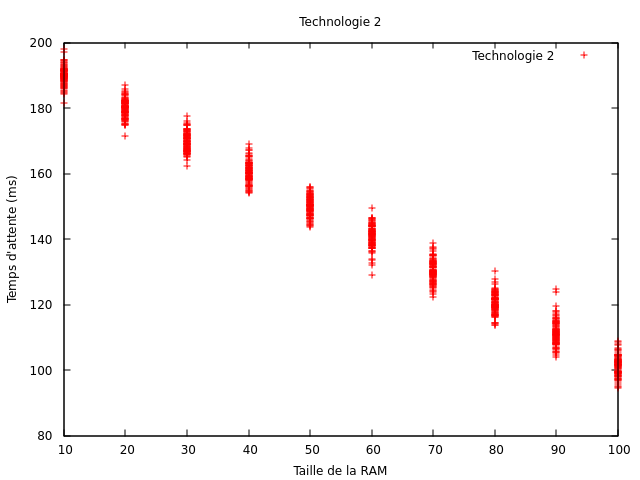
\includegraphics[scale=0.6]{img/techno2_plot.png}
\\
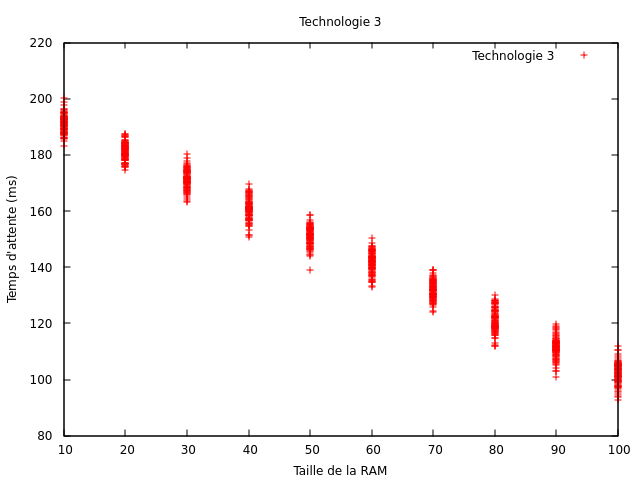
\includegraphics[scale=0.6]{img/techno3_plot.png}
\\
\\
Nous remarquons que les mesures sont très semblables pour les trois technologies. Nous allons maintenant les afficher toutes les trois sur un graphe pour voir
si l'une d'elle se démarque et semble meilleure qu'une autre.
\\
\\
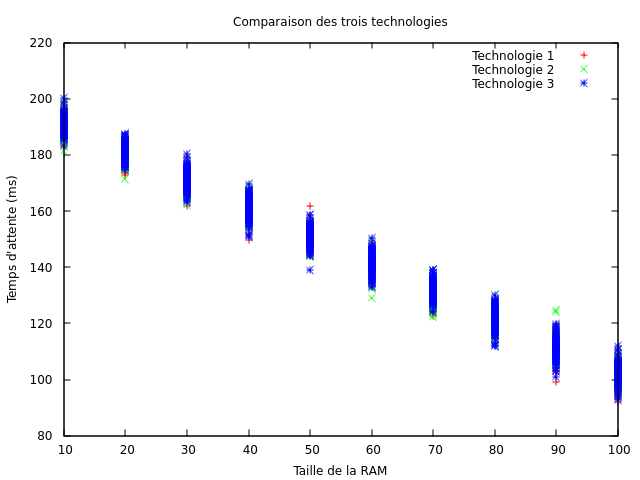
\includegraphics[scale=0.6]{img/techno_plot.png}
\\
\\
Nous remarquons que les données sont très groupées voire confondues. Nous ne pouvons pas distinguer au premier coup d'oeil de grosses différences entre les mesures observées
pour les différentes technologies. Cependant nous ne pouvons pas précisément en analyser les différence et donc dire si celles-ci sont significatives.

\section{Analyse des données}

\subsection{Histogrammes}
Nous allons visualiser nos données sous la forme d'histogrammes, ce qui va nous permettre d'observer la distribution des mesures pour chaque taille de RAM donné et pour chaque
technologie. Nous allons donc avoir un histogramme par paquet de 100 données. Nous travaillons avec des temps d'attentes qui sont des nombres flottants, nous allons donc utiliser des intervalles de temps et compter le nombre d'occurrences 
des mesures dans ces intervalles. Nous aurons donc nos intervalles en abscisse et notre nombre d'occurrences en ordonnée. Nous avons choisi d'utiliser 10 intervalles
par histogramme, ce qui nous permet de bien visualiser les données tout en ayant des nombres d'occurrences raisonnables dans chaque intervalle. Nous obtenons les
graphiques suivants : \\
\\
\subsection{Technologie n°1}
\\
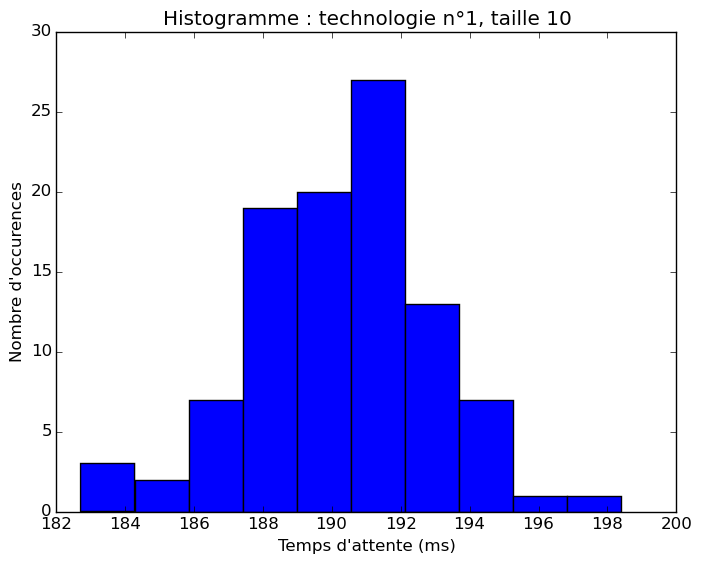
\includegraphics[scale=0.4]{img/1-10.png}
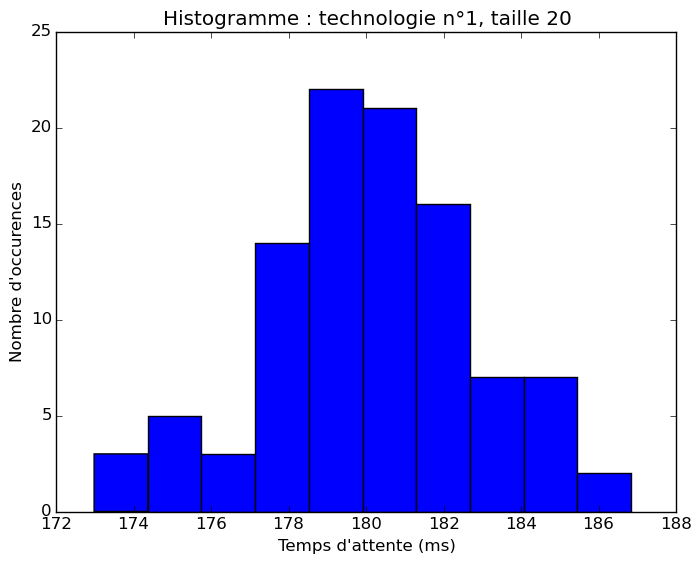
\includegraphics[scale=0.4]{img/1-20.png}
\\
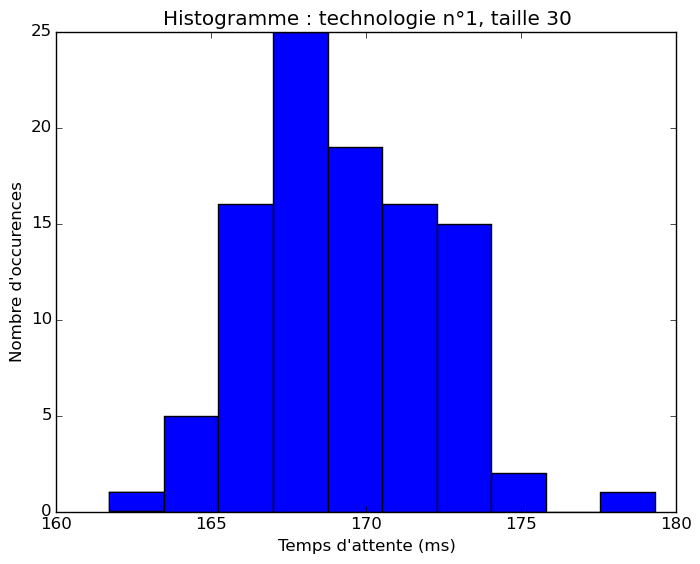
\includegraphics[scale=0.4]{img/1-30.png}
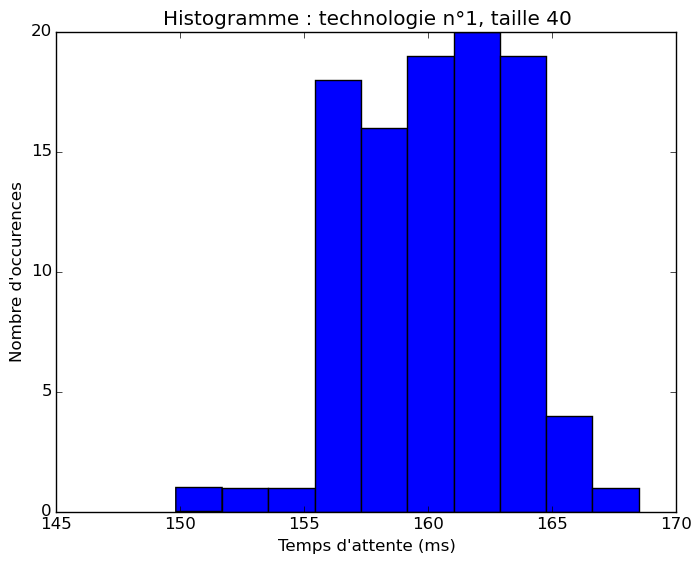
\includegraphics[scale=0.4]{img/1-40.png}
\\
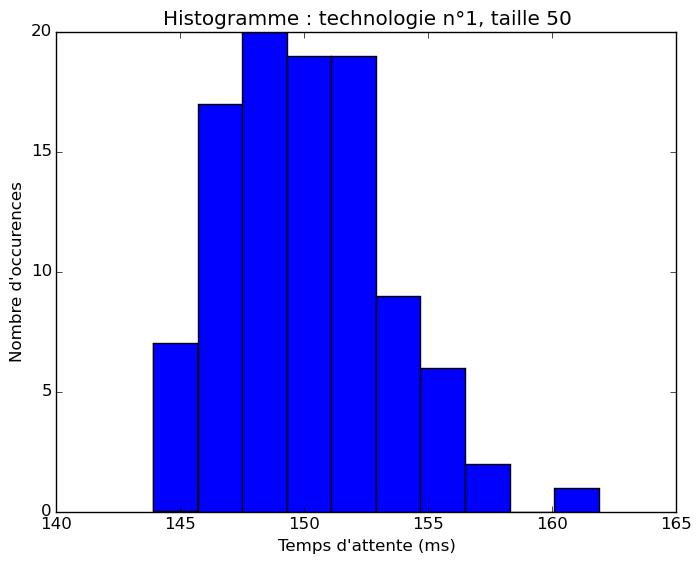
\includegraphics[scale=0.4]{img/1-50.png}
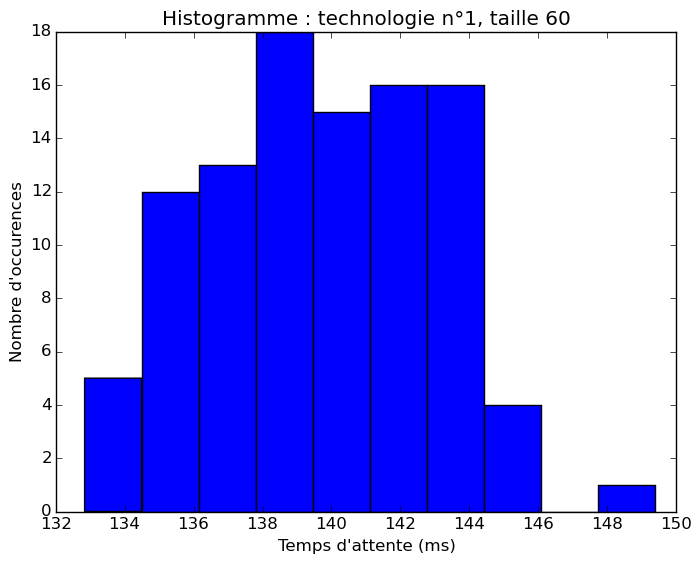
\includegraphics[scale=0.4]{img/1-60.png}
\\
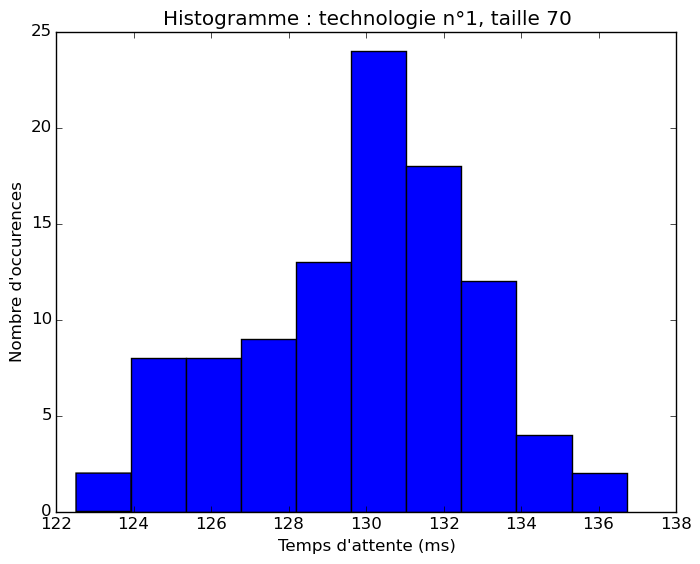
\includegraphics[scale=0.4]{img/1-70.png}
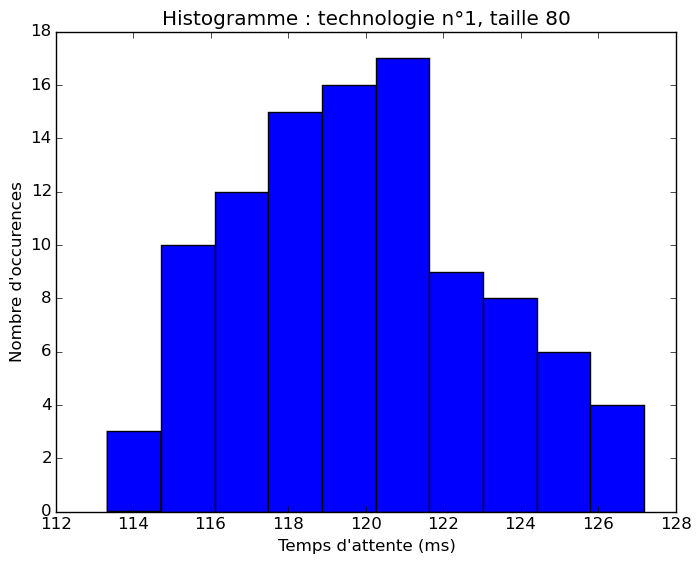
\includegraphics[scale=0.4]{img/1-80.png}
\\
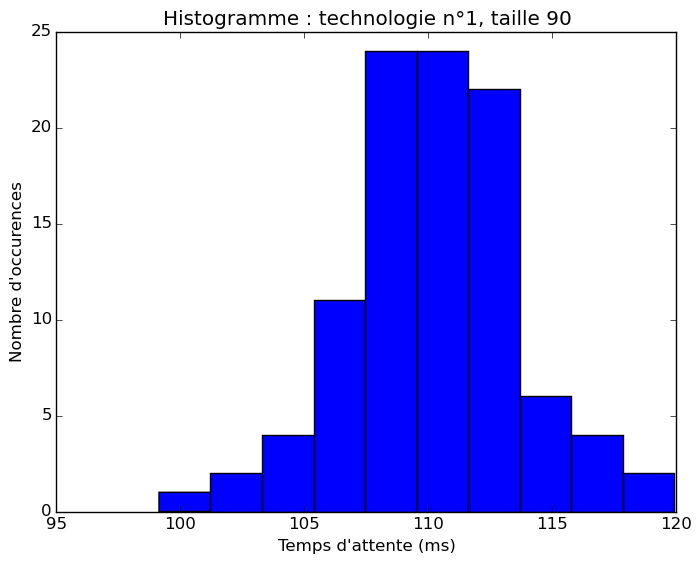
\includegraphics[scale=0.4]{img/1-90.png}
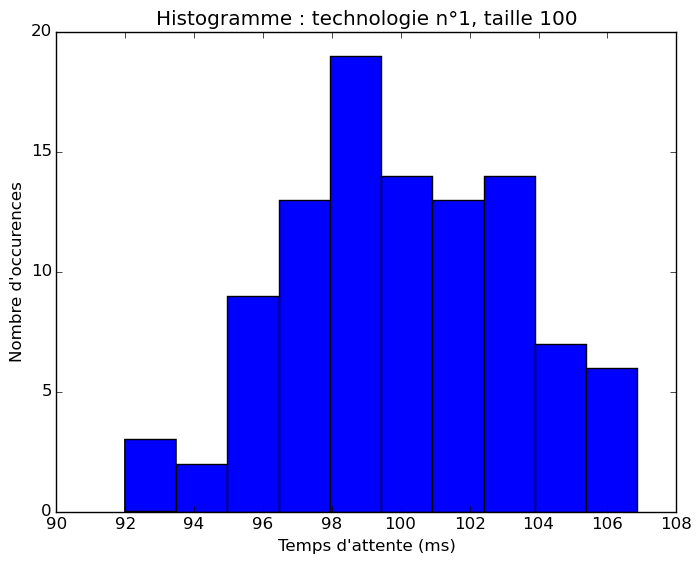
\includegraphics[scale=0.4]{img/1-100.png}
\\
\subsection{Technologie n°2}
\\
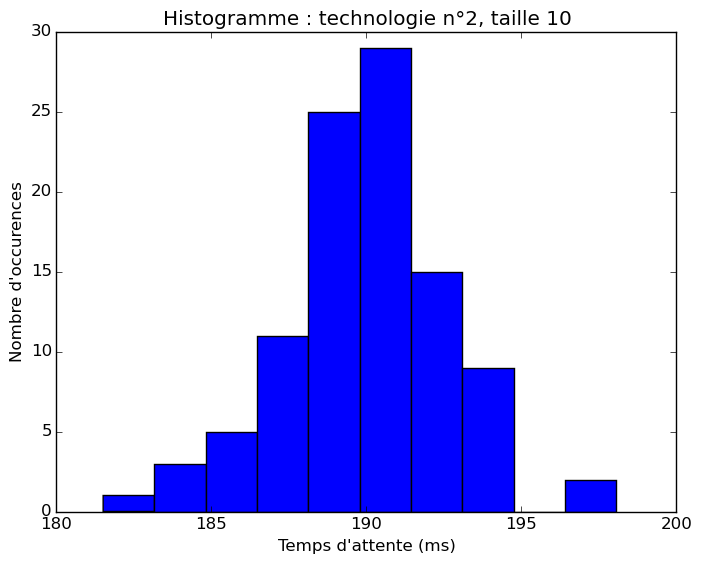
\includegraphics[scale=0.4]{img/2-10.png}
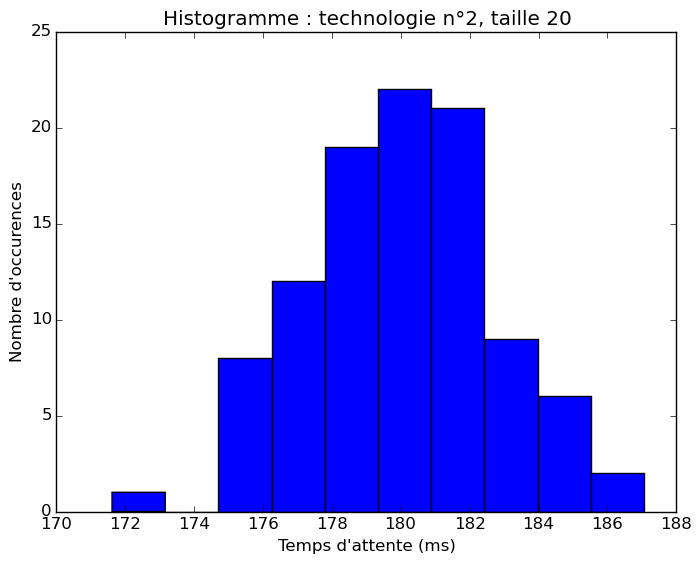
\includegraphics[scale=0.4]{img/2-20.png}
\\
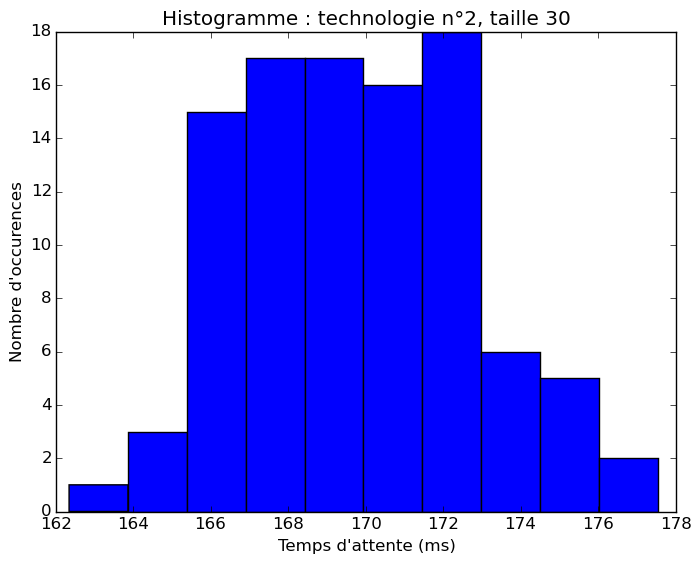
\includegraphics[scale=0.4]{img/2-30.png}
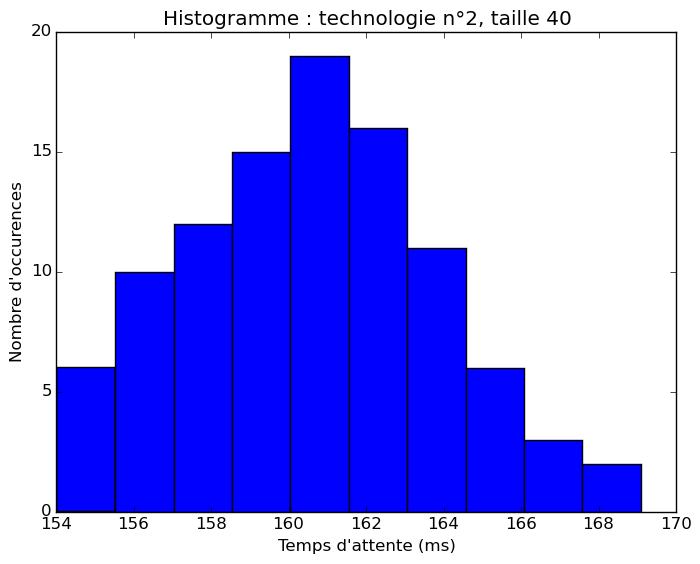
\includegraphics[scale=0.4]{img/2-40.png}
\\
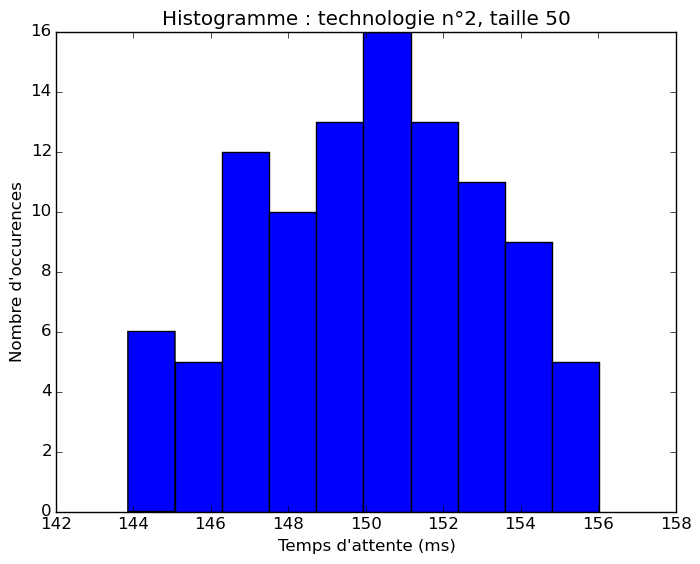
\includegraphics[scale=0.4]{img/2-50.png}
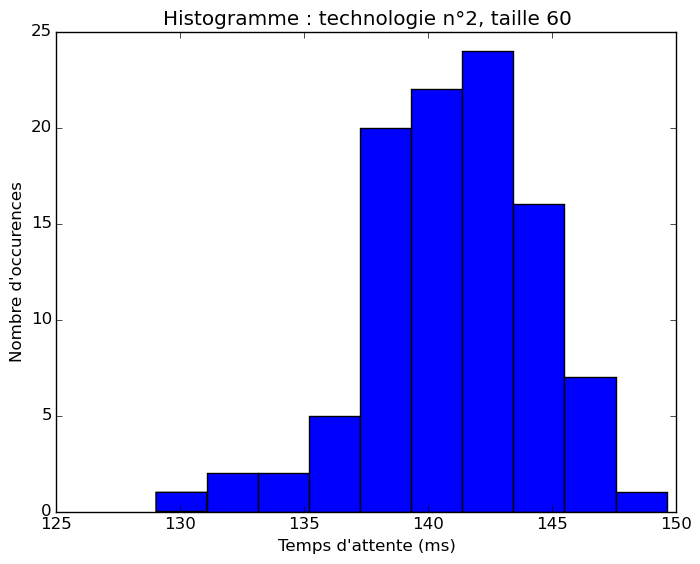
\includegraphics[scale=0.4]{img/2-60.png}
\\
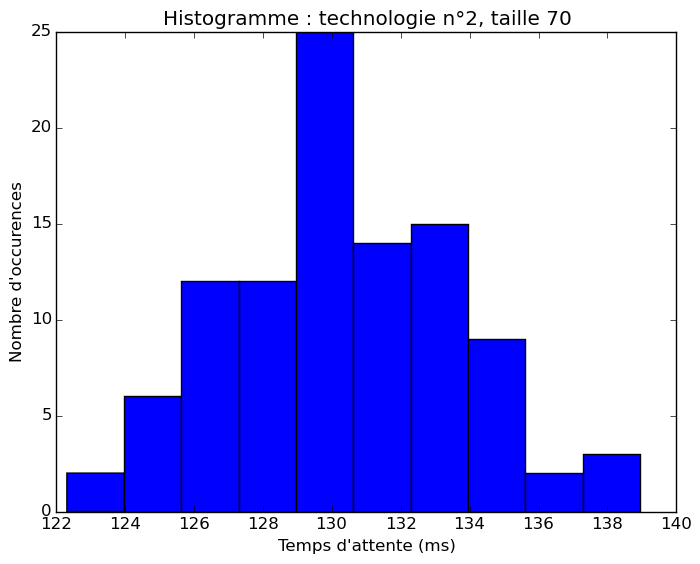
\includegraphics[scale=0.4]{img/2-70.png}
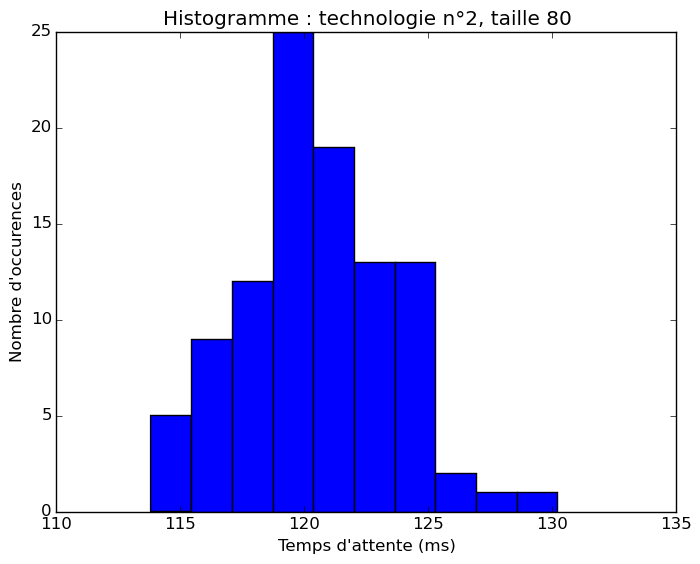
\includegraphics[scale=0.4]{img/2-80.png}
\\
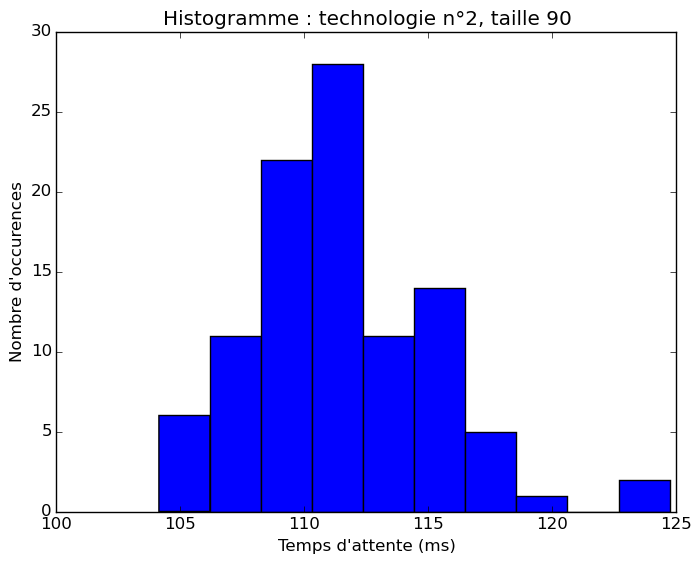
\includegraphics[scale=0.4]{img/2-90.png}
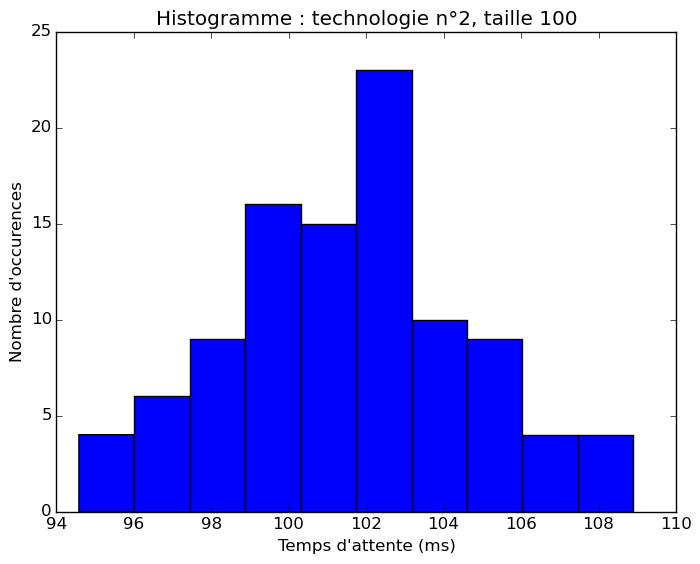
\includegraphics[scale=0.4]{img/2-100.png}
\\
\subsection{Technologie n°3}
\\
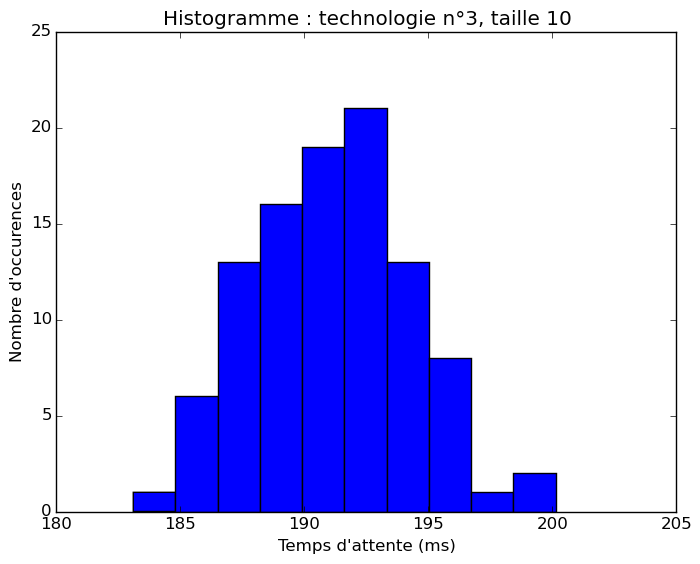
\includegraphics[scale=0.4]{img/3-10.png}
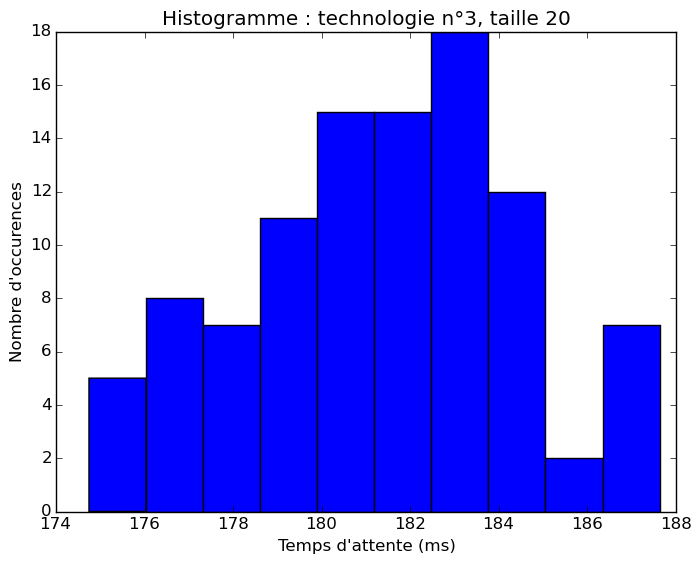
\includegraphics[scale=0.4]{img/3-20.png}
\\
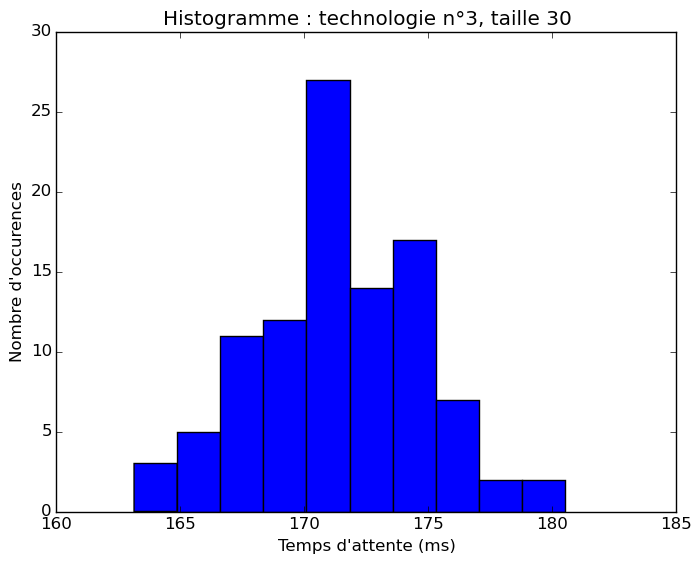
\includegraphics[scale=0.4]{img/3-30.png}
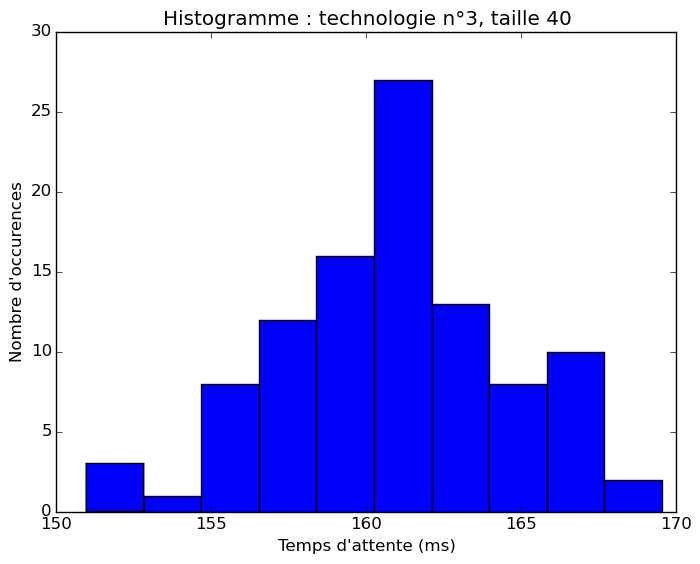
\includegraphics[scale=0.4]{img/3-40.png}
\\
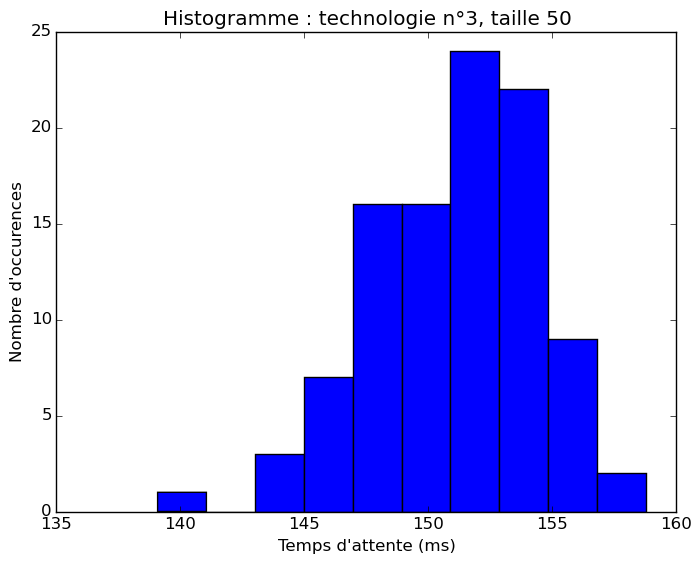
\includegraphics[scale=0.4]{img/3-50.png}
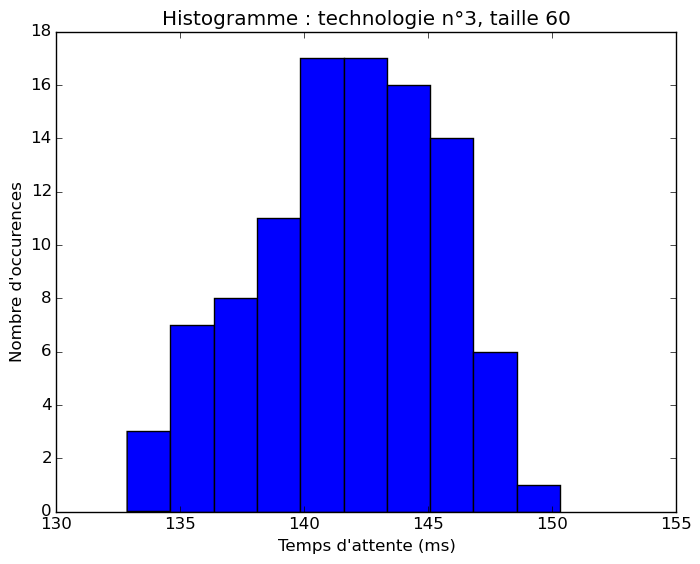
\includegraphics[scale=0.4]{img/3-60.png}
\\
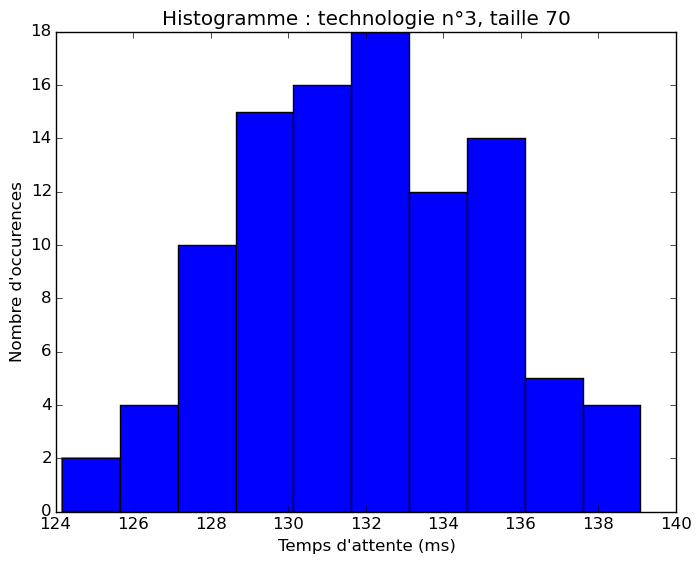
\includegraphics[scale=0.4]{img/3-70.png}
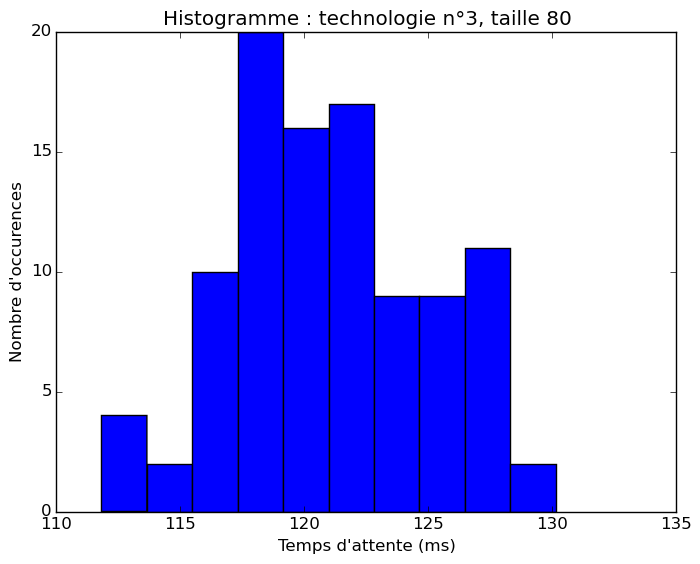
\includegraphics[scale=0.4]{img/3-80.png}
\\
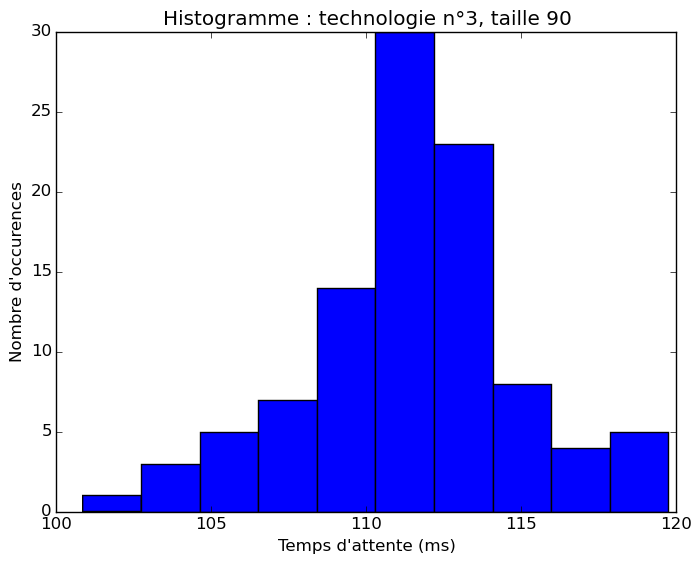
\includegraphics[scale=0.4]{img/3-90.png}
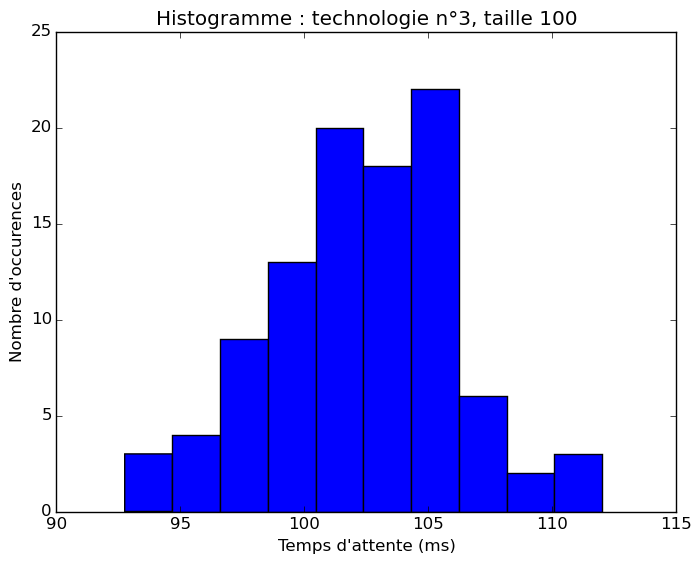
\includegraphics[scale=0.4]{img/3-100.png}
\\
\\

Nous remarquons que ces histogrammes adoptent des formes de Gaussiennes comme celles vue au cours. Ceci nous donne l'intuition que nos données
suivent une distribution Gaussienne. Nous allons estimer les paramètres de ces Gaussiennes.

\subsection{Test de loi normale}
Nos graphiques nous font penser que les données suivent des lois normales. Nous allons estimer les paramètres de ces lois grâce aux estimateurs suivants: 
\\
\begin{math}
\\
Moyenne : \mu = \sum_{i=1}^{n} \frac{1}{n}x_i \\
\\
Variance : \sigma^2 = \frac{1}{n} \sum_{i=1}^{n} (x_i - \overline{x_n})^2 \\
\end{math}
\\
Le tableau suivant regroupe les valeurs de $\mu$ et $\sigma^2$ obtenues pour chaque paquets de données : 
\\
\resizebox{\columnwidth}{!}{%
\begin{tabular}{|c|c|c|c|c|c|c|c|c|c|}
\hline
 & \multicolumn{2}{c|}{\textbf{Techno 1}} & \multicolumn{2}{c|}{\textbf{Techno 2}} & \multicolumn{2}{c|}{\textbf{Techno 3}} \\ 
\hline 
\textbf{Taille de la ram} & \textbf{$\mu$} & \textbf{$\sigma^{2}$} & \textbf{$\mu$} & \textbf{$\sigma^{2}$} & \textbf{$\mu$} & \textbf{$\sigma^{2}$} \\ 
\hline 
10 & 190.285845 & 6.83621580928 & 189.993064 & 7.0102703025 & 191.15425 & 9.7824753515 \\ 
\hline
20 & 180.176359 & 8.06744797482 & 180.031705 & 7.69889719767 & 181.349205 & 8.81349077988 \\  
\hline
30 & 169.336791 & 8.91022621842 & 169.756475 & 8.44422828047 & 171.393594 & 11.2890322504 \\
\hline
40 & 160.279539 & 10.3141003148 & 160.48538 & 10.433523362 & 160.785599 & 14.2709656719 \\  
\hline
50 & 150.120116 & 10.8529737131 & 150.090653 & 8.89111964749 & 151.095497 & 11.1139485515 \\  
\hline
60 & 139.720791 & 10.7061969092 & 140.946094 & 11.7114986398 & 141.732717 & 13.5168806338 \\ 
\hline
70 & 129.745023 & 8.68939199237 & 130.318984 & 11.1544087421 & 131.885912 & 10.4978972605 \\  
\hline
80 & 119.901673 & 9.99044969877 & 120.510974 & 9.28041881472 & 121.141859 & 16.5558357264 \\  
\hline
90 & 110.10677 & 12.7542882161 & 111.492966 & 13.8136523996 & 111.43348 & 12.2054507598 \\  
\hline
100 & 99.958019 & 10.3245662049 & 101.479214 & 9.2069703406 & 102.3378 & 13.716685828 \\  
\hline 
\end{tabular}%
}

\subsection{Test de Kolmogorov-Smirnov}
Nous voulons vérifier que nos échantillons suivent bien une loi. Cette loi est notre hypothèse nulle H_0 .
\\
Si D_n < D_$\alpha$ alors on accepte l'hypothèse nulle (on suit la loi)\\
Si D_n > D_$\alpha$ alors on refuse l'hypothèse nulle (on ne suit pas la loi)\\
\\
\begin{math}
 D_n = \frac{Sup|F_n (x)-F_0(x)|}{n}\\
\end{math}
\\
D_$\alpha$ que l'ont trouve dans les tables. \\
$F_n$ est la fonction de répartition de l'échantillon et $F_0$ est la fonction de répartition de la loi sur l'échantillon.\\
\\
Dans notre cas, n est toujours égal à 100 car nous avons des paquets de 100 données.
$D_\apha$ est donc égal à 0.134 pour une erreur de 0.05 (valeur du cours).\\
\\
Suite au test de Kolmogorov-Smirnov, nous obtenons les résultats suivants : \\
\\
\resizebox{\columnwidth}{!}{%
\begin{tabular}{|c|c|c|c|c|c|c|c|c|c|}
\hline
 & \multicolumn{2}{c|}{\textbf{Technologie 1}} & \multicolumn{2}{c|}{\textbf{Technologie 2}} & \multicolumn{2}{c|}{\textbf{Technologie 3}} \\ 
\hline 
\textbf{Taille de la ram} & \textbf{$D_n$} & \textbf{$D_\alpha$} & \textbf{$D_n$} & \textbf{$D_\alpha$} & \textbf{$D_n$} & \textbf{$D_\alpha$} \\ 
\hline 
10 & 0.0601658923615 & 0.134& 0.0687822483684 & 0.134& 0.0399246040204 & 0.134 \\                                                                                                                                                                                                  
     \hline                                                                                                                                                                                                                                                                          
20 & 0.044503791185 & 0.134& 0.0591859546793 & 0.134& 0.0533580825886 & 0.134 \\                                                                                                                                                                                                   
   \hline                                                                                                                                                                                                                                                                            
30 & 0.0721534227275 & 0.134& 0.0600413689984 & 0.134& 0.0474004732574 & 0.134\\                                                                                                                                                                                                  
 \hline                                                                                                                                                                                                                                                                              
40 & 0.0605761286224 & 0.134& 0.0435807694997 & 0.134& 0.0664836836944 & 0.134 \\                                                                                                                                                                                                  
 \hline                                                                                                                                                                                                                                                                              
50 & 0.06856718771 & 0.134& 0.0504490247843 & 0.134& 0.0571603975184 & 0.134 \\                                                                                                                                                                                                    
 \hline                                                                                                                                                                                                                                                                              
60 & 0.0844704309149 & 0.134& 0.0447916372736 & 0.134& 0.0503350632265 & 0.134 \\                                                                                                                                                                                                  
  \hline                                                                                                                                                                                                                                                                             
70 & 0.103542660509 & 0.134& 0.052023677948 & 0.134& 0.0595021117656 & 0.134 \\                                                                                                                                                                                                    
   \hline                                                                                                                                                                                                                                                                            
80 & 0.068536709881 & 0.134& 0.0561637285433 & 0.134& 0.0827458283825 & 0.134 \\                                                                                                                                                                                                   
   \hline                                                                                                                                                                                                                                                                            
90 & 0.0587333056383 & 0.134& 0.0873489528759 & 0.134& 0.0846705839 & 0.134 \\                                                                                                                                                                                                     
   \hline                                                                                                                                                                                                                                                                            
100 & 0.0492695131459 & 0.134& 0.0575043579993 & 0.134& 0.0639172664981 & 0.134 \\
\hline 
\end{tabular}%
}

Nous remarquons que les tests sont toujours réussis pour les trois technologies. Nous en concluons que les trois technologies suivent une loi normale.

\subsection{Test de Fisher-Snedecor}
Rappels théoriques : \\

Soient deux échantillons gaussiens X($\mu_x$,$\sigma_x^2$,$n_x$) et Y($\mu_y$,$\sigma_y^2$,$n_y$) où $\sigma_x^2$ $>$ $\sigma_y^2$.\\
On suppose l'hypothèse nulle $H_0$ : $\sigma_x^2$ = $\sigma_y^2$ \\
Soit \\
\\
\begin{math}
T = \frac{ \frac{n_x}{n_x-1} \sigma_x^2}{ \frac{n_y}{n_y-1} \sigma_y^2}
\end{math}
\\
\\
Si T $<$ $F_{\alpha/2}$ on accepte l'hypothèse nulle avec $F_{\alpha/2}$ la valeur de la loi de Fisher-Snedecor et $\alpha$ l'erreur de première espèce.\\
Notre erreur de première espèce utilisée est 0.05 comme précédemment utilisé dans le test de Kolmogorov. Notre valeur de $F_{\alpha/2}$ est donc 1.48\\
\\
Les résultats des tests de Fisher-Snedecor sont les suivants : \\
\\
\resizebox{\columnwidth}{!}{%
\begin{tabular}{|c|c|c|c|c|c|c|c|c|c|}
\hline
 & \multicolumn{2}{c|}{\textbf{Technologie 1 - 2}} & \multicolumn{2}{c|}{\textbf{Technologie 2 - 3}} & \multicolumn{2}{c|}{\textbf{Technologie 1 - 3}} \\ 
\hline 
\textbf{Taille de la ram} & \textbf{T} & \textbf{$F_{\alpha/2$}} & \textbf{T} & \textbf{$F_{\alpha/2}$} & \textbf{T} & \textbf{$F_{\alpha/2}$} \\ 
\hline 
10 & 1.0254606493 & 1.48 &  1.39544909531 & 1.48 &  1.43097813533 & 1.48   \\                                                                                                                                                                                                      
\hline 
20 & 1.04787059337 & 1.48 &  1.14477314784 & 1.48 &  1.09247568839 & 1.48   \\
\hline 
30 & 1.05518537899 & 1.48 &  1.33689330456 & 1.48 &  1.266974819 & 1.48   \\
\hline 
40 & 1.01157861991 & 1.48 &  1.36779927324 & 1.48 &  1.38363650114 & 1.48   \\
\hline 
50 & 1.22065320718 & 1.48 &  1.25000551023 & 1.48 &  1.02404638998 & 1.48   \\
\hline 
60 & 1.09389905109 & 1.48 &  1.15415465173 & 1.48 &  1.26252867834 & 1.48   \\
\hline 
70 & 1.28368115421 & 1.48 &  1.06253742682 & 1.48 &  1.20812794148 & 1.48   \\
\hline 
80 & 1.07650849581 & 1.48 &  1.78395351082 & 1.48 &  1.6571662163 & 1.48  \\
\hline 
90 & 1.0830594515 & 1.48 &  1.13176093792 & 1.48 &  1.04496658641 & 1.48   \\
\hline 
100 & 1.12138584388 & 1.48 &  1.48981535951 & 1.48 &  1.32854839184 & 1.48   \\
\hline 
\end{tabular}%
}
\\
\\
Nous remarquons le nombre suivant de résultats ``vrai'' (sur 10 tests) pour l'équation T $<$ $F_{\alpha/2}$ :\\ \\
\begin{tabular}{|c|c|c|}
\hline
Technologie 1 - 2 & Technologie 2 - 3 & Technologie 1 - 3 \\
\hline
10 & 8 & 9 \\
\hline
\end{tabular}
\\
\\
Nous en concluons que l'hypothèse nulle est vraie et que les variances des trois technologies sont égales.\\
Ce résultat nous permet d'effectuer un test de moyenne.

\subsection{Test de moyenne}
Si l’inégalité suivante est vérifiée alors on peut conclure que les moyennes sont différentes : \\

$|\mu_1$ - $\mu_2 |$ $>$ $Z_{1-\alpha/2}$ $\sqrt[2]{ \frac{\sigma_1^2}{n_1}+\frac{\sigma_2^2}{n_2} }$ \\
\\
Dans notre cas, nous avons une valeur de $\alpha$ = 0.05 et donc de $Z_{1-\alpha/2}$ = 1.96.\\
\\
Nous observons les résultats suivants :\\
\\
\resizebox{\columnwidth}{!}{%
\begin{tabular}{|c|c|c|c|c|c|c|c|c|c|}
\hline
 & \multicolumn{2}{c|}{\textbf{Technologie 1 - 2}} & \multicolumn{2}{c|}{\textbf{Technologie 2 - 3}} & \multicolumn{2}{c|}{\textbf{Technologie 1 - 3}} \\ 
\hline 
\textbf{Taille de la ram} & \textbf{$|\mu_1$ - $\mu_2 |$} & \textbf{$Z_{1-\alpha/2}$ $\sqrt[2]{ \frac{\sigma_1^2}{n_1}+\frac{\sigma_2^2}{n_2} }$} & \textbf{$|\mu_1$ - $\mu_2 |$} & \textbf{$Z_{1-\alpha/2}$ $\sqrt[2]{ \frac{\sigma_1^2}{n_1}+\frac{\sigma_2^2}{n_2} }$} & \textbf{$|\mu_1$ - $\mu_2 |$} & \textbf{$Z_{1-\alpha/2}$ $\sqrt[2]{ \frac{\sigma_1^2}{n_1}+\frac{\sigma_2^2}{n_2} }$} \\ 
\hline 
10 & 0.292781 & 0.729332990115 &  1.161186 & 0.803187473162 &  0.868405 & 0.799014167354   \\
\hline 
20 & 0.144654 & 0.77825440323 &  1.3175 & 0.796454579085 &  1.172846 & 0.805293824141   \\
\hline 
30 & 0.419684 & 0.816510088137 &  1.637119 & 0.870673840512 &  2.056803 & 0.880894269102   \\
\hline 
40 & 0.205841 & 0.892771365562 &  0.300219 & 0.974190767112 &  0.50606 & 0.971833264992   \\
\hline 
50 & 0.029463 & 0.870912791583 &  1.004844 & 0.876649701952 &  0.975381 & 0.918630113657   \\
\hline 
60 & 1.225303 & 0.928007646633 &  0.786623 & 0.9844660574 &  2.011926 & 0.964652137764   \\
\hline 
70 & 0.573961 & 0.873109070516 &  1.566928 & 0.912027953188 &  2.140889 & 0.858544642949   \\
\hline 
80 & 0.609301 & 0.860412508518 &  0.630885 & 0.996255767588 &  1.240186 & 1.00985251443  \\
\hline 
90 & 1.386196 & 1.01026432516 &  0.059486 & 0.999774908153 &  1.32671 & 0.979210565965  \\
\hline 
100 & 1.521195 & 0.86621216104 &  0.858586 & 0.938421640508 &  2.379781 & 0.961024837399  \\
\hline 
\end{tabular}%
}
\\
\\
Nous obtenons les résultats suivants pour la véracité de l'équation :\\
\\
\begin{tabular}{|c|c|c|}
\hline
Technologie 1 - 2 & Technologie 2 - 3 & Technologie 1 - 3 \\
\hline
False & True & True \\
\hline
False& True& True \\
\hline
False &True &True \\
\hline
False& False& False \\
\hline
False &True& True \\
\hline
True &False &True \\
\hline
False &True& True \\
\hline
False& False& True \\
\hline
True& False& True \\
\hline
True &False& True \\
\hline
\end{tabular}
\\
Pour les technologies 1 et 2, nous remarquons une majorité de ``False'' ce qui nous permet de dire que les moyennes sont égales. Pour les technologies 2 et 3,
nous remarquons une égalité de ``True'' et de ``False'' ce qui nous fait penser que ces deux technologies ont des moyennes différentes pour certaines tailles et 
égales pour d'autres tailles de RAM. Pour les technologies 1 et 3, nous remarquons une majorité de ``True'' donc les moyennes sont différentes.
\\
Ceci nous permet de dire que pour les technologies 1 et 2, les droites seront similaires et proches l'une de l'autre. Pour les technologies 2 et 3 aussi. Cependant
on remarquera une plus grosse différence entre les droites des technologies 1 et 3.
\subsection{Régression linéaire}
Nous allons maintenant déterminer si il est possible d'approximer les données avec une droite d'équation f(x) = ax+b pour chaque technologie.
Nous allons pour cela utiliser les fonctions fit et stat de gnuplot. Nous allons obtenir le coefficient de corrélation R² qui nous donne la qualité de la régression
Plus celui-ci est proche de 1, plus la qualité de la régression est élevée.
Nous observons les régressions suivantes : \\





Nous voyons que le (ordre de rapidité)

NOus en concluons
\end{document}
